\documentclass[10pt]{beamer}
\usepackage{ceai-beamer}
\usepackage{ragged2e}
\usepackage{amsmath,amssymb}
\usepackage{graphicx}
\usepackage{tikz}
\usepackage{bm}
\usepackage{hyperref}

\graphicspath{{../figs/}{./figs/}}

\title[Topic 6]{CE 488/5588: Applied Machine Learning\\\large Topic 6: Support Vector Machines}
\author{}
\date{}

\begin{document}

\begin{frame}[plain]
  \titlepage
\end{frame}

\begin{frame}{Outline}
  \justifying
  \tableofcontents
\end{frame}

\section{Introduction}

\begin{frame}{Why Study SVMs?}
  \justifying
  \begin{itemize}
    \item SVMs are margin-based models grounded in statistical learning theory.
    \item They often provide strong baseline performance in classification.
    \item They control capacity explicitly through regularization.
  \end{itemize}
  \vspace{0.4em}
  \footnotesize
  Sources: \href{https://see.stanford.edu/materials/aimlcs229/cs229-notes3.pdf}{Stanford CS229 Notes},
  \href{https://link.springer.com/article/10.1023/A:1022627411411}{Cortes\&Vapnik (1995)}
\end{frame}

\begin{frame}{From Topic 5 to Topic 6}
  \justifying
  \begin{itemize}
    \item Topic 5 emphasized ANN expressiveness and training dynamics.
    \item SVMs emphasize geometric separation with controlled complexity.
    \item The key bridge is generalization under limited data.
  \end{itemize}
\end{frame}

\begin{frame}{Learning Objectives}
  \justifying
  After this topic, you should be able to:
  \begin{itemize}
    \item Explain boundary, margin, and support vectors.
    \item Derive linear SVM objective terms and their roles.
    \item Interpret hinge loss and soft-margin constraints.
    \item Explain kernel trick and common kernels.
    \item Relate SVM regularization to VC-style generalization thinking.
  \end{itemize}
\end{frame}

\begin{frame}{Historical Context of SVM}
  \justifying
  \begin{itemize}
    \item Statistical Learning Theory predates modern deep learning.
    \item SVM formulation matured in the early 1990s.
    \item Vapnik's work heavily shaped margin-based learning.
  \end{itemize}
  \vspace{0.4em}
  \footnotesize
  Sources: \href{https://web.mit.edu/6.034/wwwbob/svm-notes-long-08.pdf}{MIT 6.034 Notes},
  \href{https://link.springer.com/article/10.1023/A:1022627411411}{Machine Learning (1995)}
\end{frame}

\begin{frame}{When SVM is a Strong First Choice}
  \justifying
  \begin{examplebox}{Practical Positioning}
    \begin{itemize}
      \item Medium-sized tabular data with clear class structure.
      \item High-dimensional feature spaces with careful regularization.
      \item Benchmarking before deploying more complex pipelines.
    \end{itemize}
  \end{examplebox}
\end{frame}

\section{Notations and Preliminaries}

\begin{frame}{Training Set Notation}
  \justifying
  We use
  \[
    \mathcal{D} = \{(\bm{x}_i,y_i) \mid i=1,\ldots,N;\ \bm{x}_i\in\mathbb{R}^D,\ y_i\in\{-1,1\}\}.
  \]
  \begin{itemize}
    \item $D$ is feature dimension.
    \item $N$ is number of training samples.
  \end{itemize}
\end{frame}

\begin{frame}{Decision Function Form}
  \justifying
  \begin{conceptbox}{Classifier Decomposition}
    \begin{itemize}
      \item Decision function: $u(\bm{x})$.
      \item Label rule: $f[u(\bm{x})]=\mathrm{Sign}(u(\bm{x}))$.
      \item Boundary: $u(\bm{x})=0$.
    \end{itemize}
  \end{conceptbox}
\end{frame}

\begin{frame}{Linear Parameterization}
  \justifying
  \[
    u(\bm{x}) = w_1x_1 + \cdots + w_Dx_D + b = \langle\bm{w},\bm{x}\rangle + b.
  \]
  \begin{itemize}
    \item $\bm{w}$ controls orientation.
    \item $b$ shifts the hyperplane.
  \end{itemize}
\end{frame}

\begin{frame}{Sign Rule and Binary Decision}
  \justifying
  \begin{itemize}
    \item If $u(\bm{x})\ge 0$, predict $+1$.
    \item If $u(\bm{x})<0$, predict $-1$.
  \end{itemize}
  \begin{warningbox}{Optimization Note}
    The sign function is non-differentiable, so direct minimization is replaced
    by convex surrogates such as hinge loss.
  \end{warningbox}
\end{frame}

\begin{frame}{Absorbing Bias into Augmented Vector}
  \justifying
  Define $x_0=1$ and $w_0=b$:
  \[
    u(\bm{x}) = \langle\bm{w}',\bm{x}'\rangle,
    \quad
    \bm{x}'=[x_0,x_1,\ldots,x_D]^T.
  \]
\end{frame}

\begin{frame}{Geometry in 2D}
  \justifying
  \begin{figure}[ht]
    \centering
    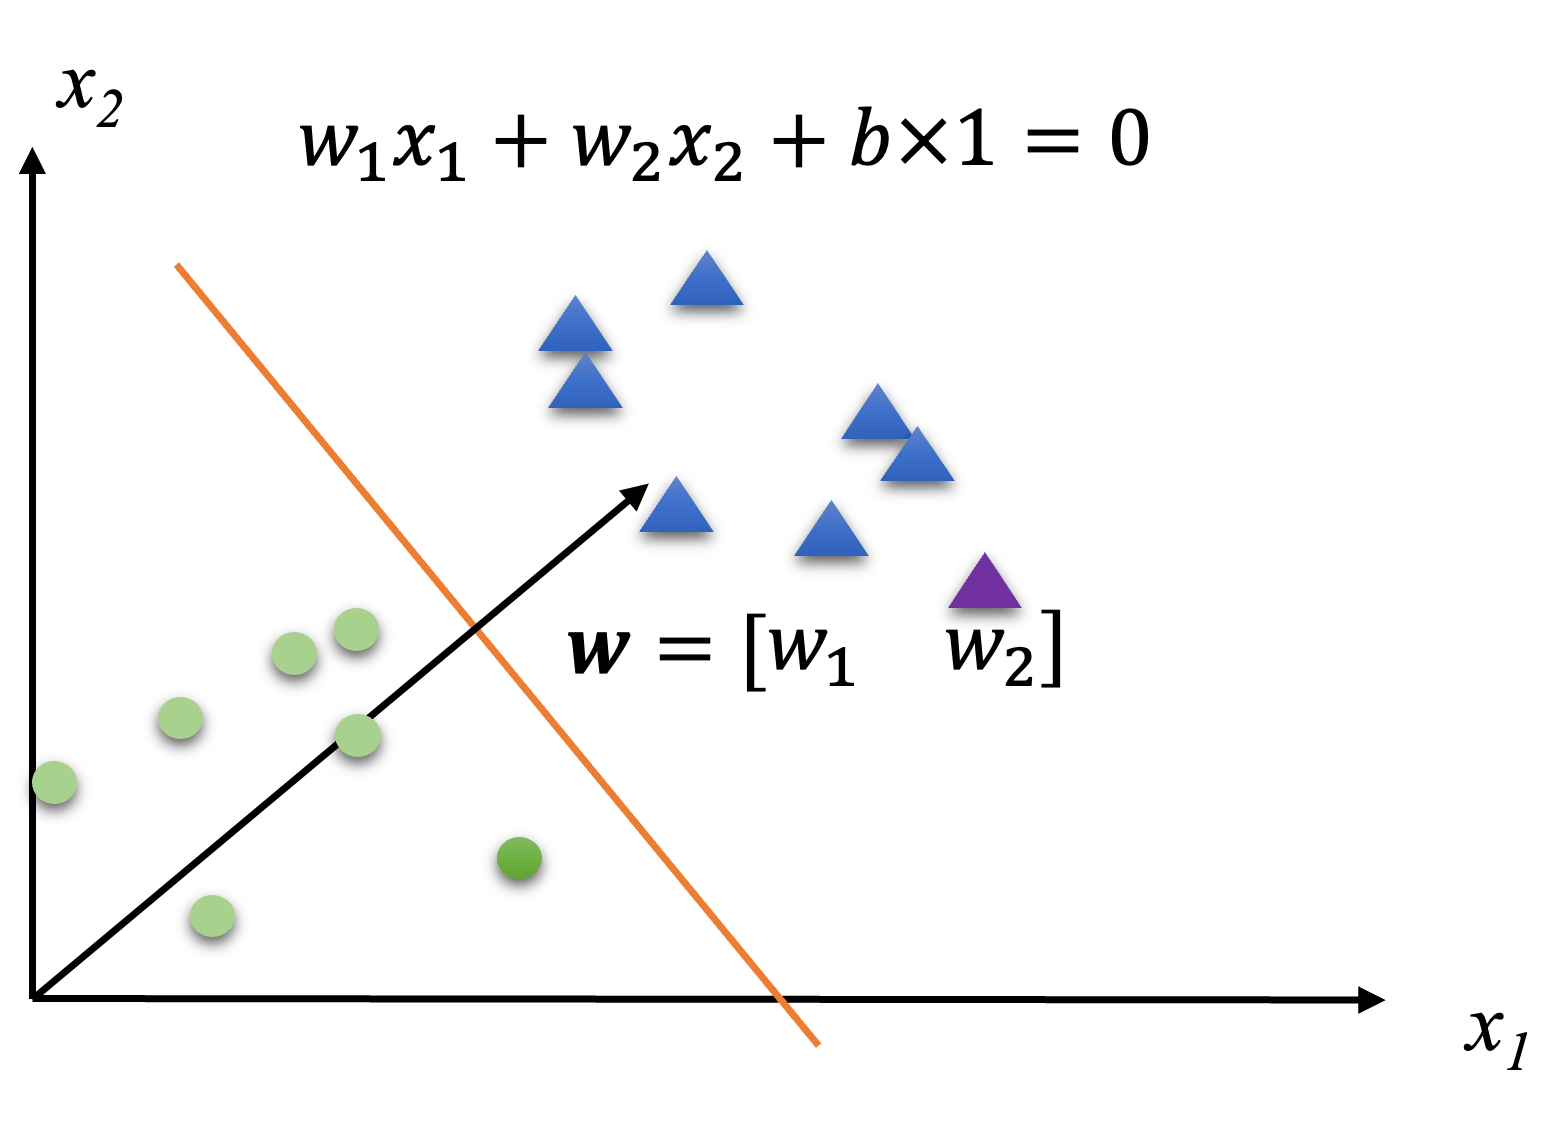
\includegraphics[width=0.62\textwidth]{Topic06fig01.png}
    \caption{Linear decision boundary $u(\bm{x})=0$ and its normal vector $\bm{w}$.}
  \end{figure}
\end{frame}

\begin{frame}{Orthogonality Intuition}
  \justifying
  \begin{itemize}
    \item The boundary slope in 2D is $-w_1/w_2$.
    \item The direction slope of $\bm{w}$ is $w_2/w_1$.
    \item Product equals $-1$, so they are orthogonal.
  \end{itemize}
\end{frame}

\section{Linear SVM Formulation}

\begin{frame}{Why Minimize More Than Training Error?}
  \justifying
  \begin{itemize}
    \item Zero training loss can still produce poor test behavior.
    \item Multiple separators may fit separable data equally well.
    \item We need a tie-breaker tied to generalization.
  \end{itemize}
\end{frame}

\begin{frame}{Decision Margins}
  \justifying
  Define two margin planes:
  \[
    \langle\bm{w},\bm{x}\rangle+b=1,
    \qquad
    \langle\bm{w},\bm{x}\rangle+b=-1.
  \]
  They are parallel to $u(\bm{x})=0$.
\end{frame}

\begin{frame}{Margin Figure for Separable Data}
  \justifying
  \begin{figure}[ht]
    \centering
    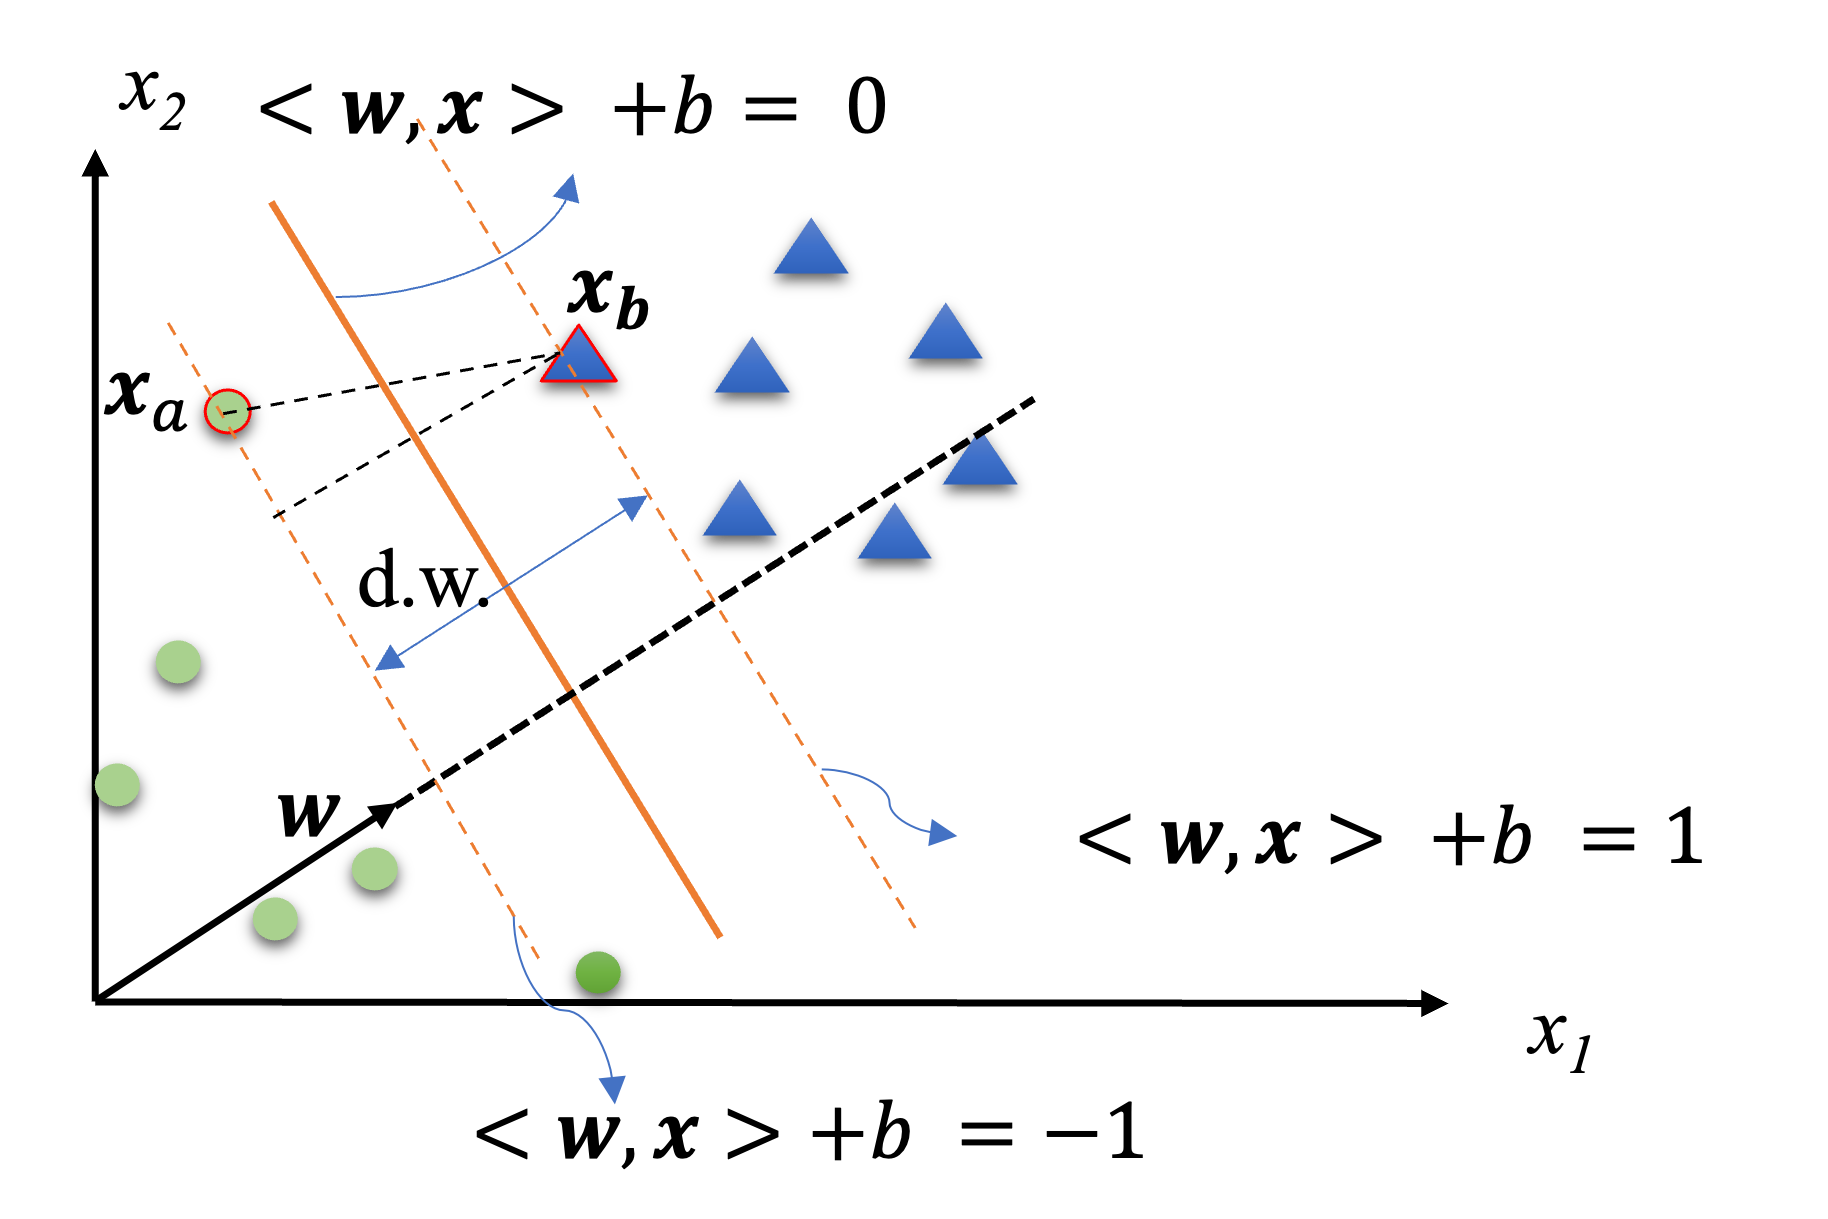
\includegraphics[width=0.62\textwidth]{Topic06fig02.png}
    \caption{Linear SVM margins and boundary in separable data.}
  \end{figure}
\end{frame}

\begin{frame}{Support Vectors and Margin Width}
  \justifying
  \begin{conceptbox}{Key Geometry}
    \begin{itemize}
      \item Support vectors are closest points to the decision boundary.
      \item Margin width is the distance between the two margin planes.
      \item Wider margin generally implies better robustness.
    \end{itemize}
  \end{conceptbox}
\end{frame}

\begin{frame}{Deriving Decision Width}
  \justifying
  \[
    \text{width} = \frac{\langle\bm{x}_b-\bm{x}_a,\bm{w}\rangle}{\|\bm{w}\|}
    = \frac{2}{\|\bm{w}\|}.
  \]
  Hence maximizing width is equivalent to minimizing $\|\bm{w}\|$.
\end{frame}

\begin{frame}{Complexity View of $\|\bm{w}\|^2$}
  \justifying
  \begin{itemize}
    \item Small $\|\bm{w}\|^2$ means larger margin.
    \item Larger margin reduces sensitivity to perturbations.
    \item This is a practical proxy for complexity control.
  \end{itemize}
\end{frame}

\begin{frame}{Regularized Learning Objective}
  \justifying
  \[
    L(\bm{w}) = \frac{1}{N}\sum_{i=1}^N l_i + \|\bm{w}\|^2.
  \]
  \begin{itemize}
    \item First term favors fit.
    \item Second term favors margin and lower complexity.
  \end{itemize}
\end{frame}

\begin{frame}{Trade-Off Visualization}
  \justifying
  \begin{figure}[ht]
    \centering
    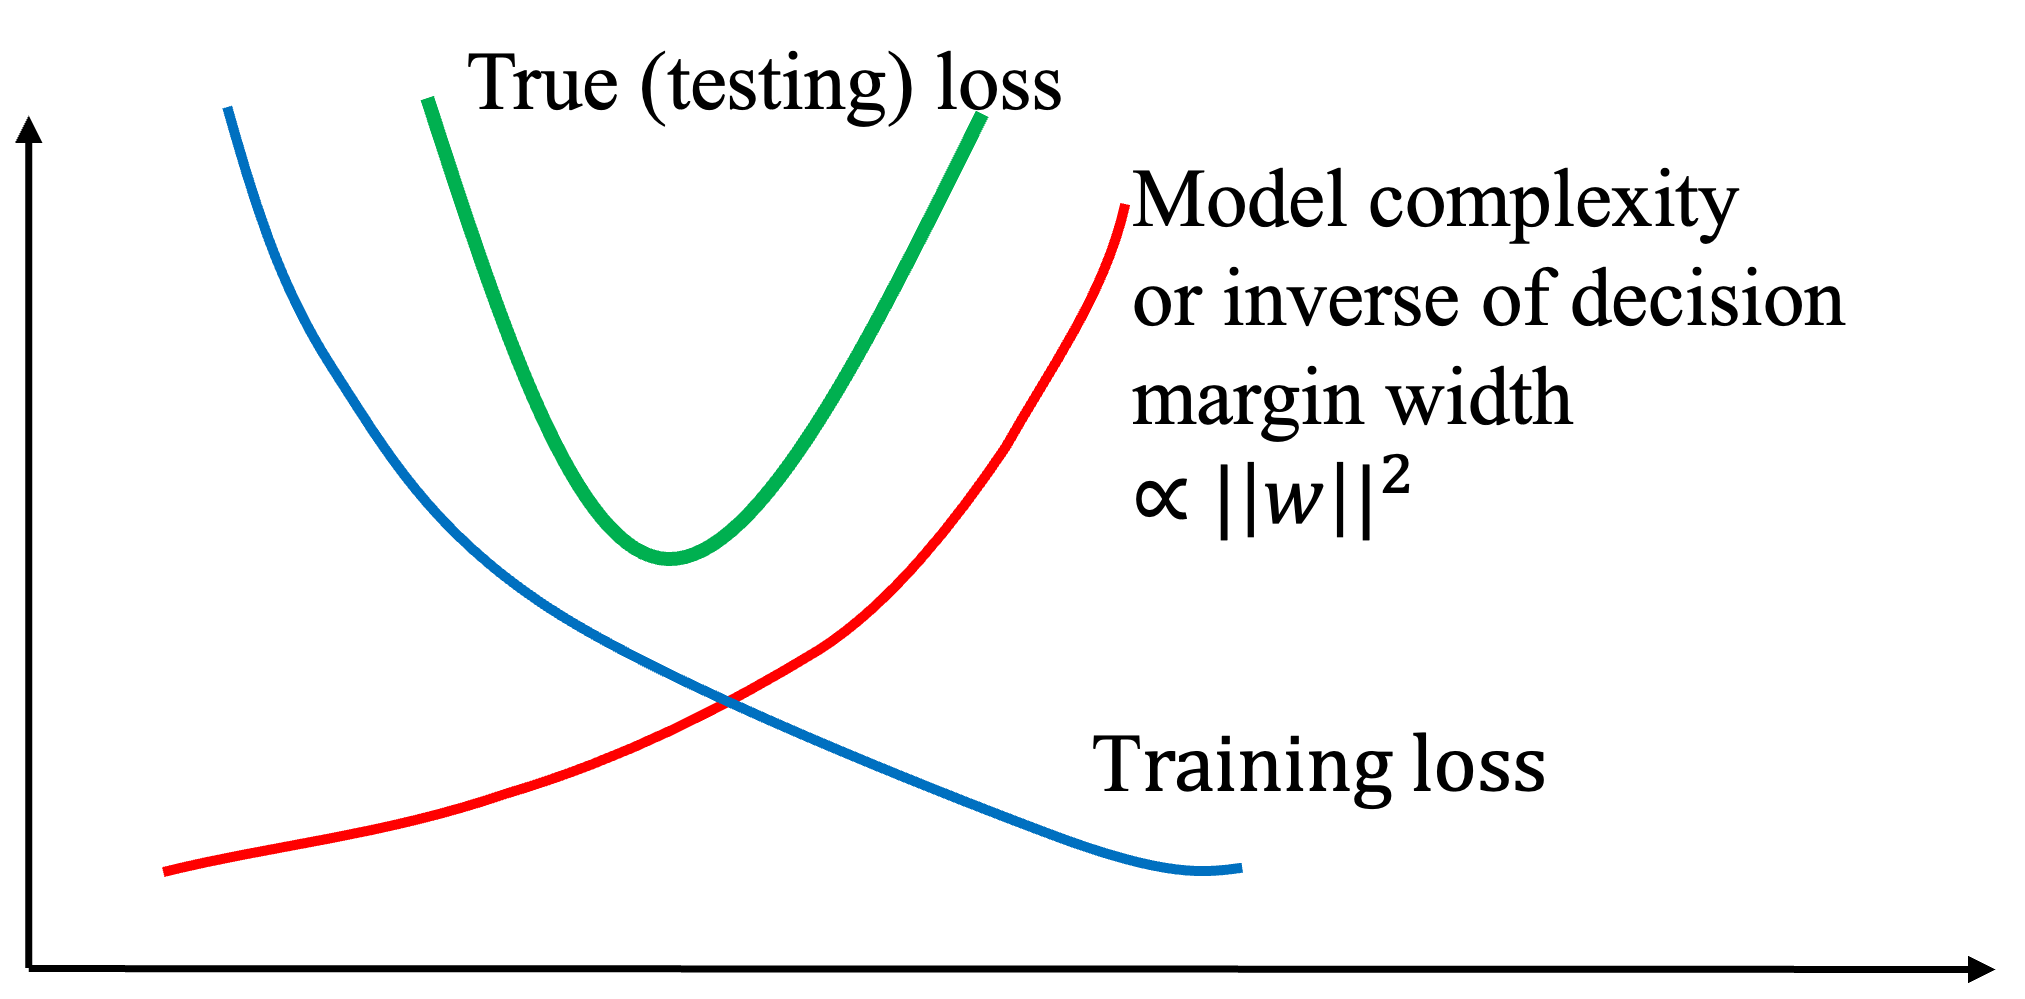
\includegraphics[width=0.62\textwidth]{Topic06fig03.png}
    \caption{Balancing training loss and model complexity for testing performance.}
  \end{figure}
\end{frame}

\begin{frame}{Interpretation of the Trade-Off Curve}
  \justifying
  \begin{itemize}
    \item Underfitting region: high bias, low complexity.
    \item Overfitting region: low training error but high complexity.
    \item Preferred region: balanced true risk.
  \end{itemize}
\end{frame}

\begin{frame}{Single-Item Principle: Margin as Core Criterion}
  \justifying
  \begin{itemize}
    \item Margin maximization is the central SVM design idea.
    \begin{itemize}
      \item It resolves non-uniqueness among many separators.
      \item It gives a direct mechanism for generalization control.
      \item It aligns geometric intuition with optimization objectives.
    \end{itemize}
  \end{itemize}
\end{frame}

\section{Hinge Loss and Soft Margin}

\begin{frame}{From Separable to Non-Separable Data}
  \justifying
  \begin{itemize}
    \item Most real datasets are not perfectly linearly separable.
    \item Some samples must violate margin constraints.
    \item The objective should penalize, not forbid, these violations.
  \end{itemize}
\end{frame}

\begin{frame}{Hinge Loss Definition}
  \justifying
  \[
    h_i = \max\bigl(0,\ 1-y_i u(\bm{x}_i)\bigr).
  \]
  \vspace{0.3em}
  \footnotesize
  Source: \href{https://see.stanford.edu/materials/aimlcs229/cs229-notes3.pdf}{Stanford CS229 Notes}
\end{frame}

% \begin{frame}{Hinge Loss Shape}
%   \justifying
%   Let $u=u(\bm{x}_i)$. The hinge loss is $h=\max(0,1-y_i u)$.
%   \vspace{0.3em}

%   \centering
%   \begin{tikzpicture}[scale=0.85]
%     % axes
%     \draw[->] (-3.2,0) -- (3.2,0) node[right] {$u$};
%     \draw[->] (0,-0.2) -- (0,3.0) node[above] {$h$};

%     % y=+1: h = max(0, 1-u)
%     \draw[very thick, blue] (-3,4) -- (1,0);
%     \draw[very thick, blue] (1,0) -- (3,0);
%     \node[blue] at (2.1,1.6) {$y_i=+1$};

%     % y=-1: h = max(0, 1+u)
%     \draw[very thick, red] (-3,0) -- (-1,0);
%     \draw[very thick, red] (-1,0) -- (3,4);
%     \node[red] at (-2.0,1.6) {$y_i=-1$};

%     % margin points
%     \fill (1,0) circle (1.4pt);
%     \fill (-1,0) circle (1.4pt);
%     \node[below] at (1,0) {$1$};
%     \node[below] at (-1,0) {$-1$};
%   \end{tikzpicture}
% \end{frame}

\begin{frame}{Hinge Loss Shape}
  \justifying
  Let $u=u(\bm{x}_i)$. The hinge loss is $h=\max(0,1-y_i u)$.
  \vspace{0.3em}

  \centering
  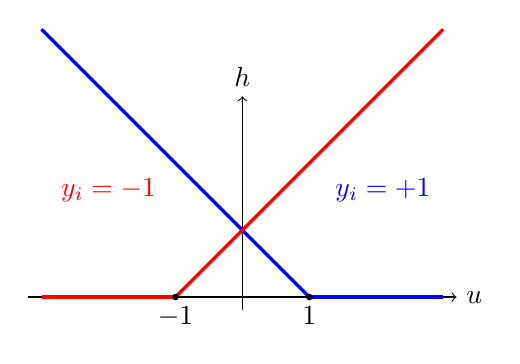
\begin{tikzpicture}[scale=0.85]
    % axes
    \draw[->] (-3.2,0) -- (3.2,0) node[right] {$u$};
    \draw[->] (0,-0.2) -- (0,3.0) node[above] {$h$};

    % y=+1: h = max(0, 1-u)
    \draw[very thick, blue] (-3,4) -- (1,0);
    \draw[very thick, blue] (1,0) -- (3,0);
    \node[blue] at (2.1,1.6) {$y_i=+1$};

    % y=-1: h = max(0, 1+u)
    \draw[very thick, red] (-3,0) -- (-1,0);
    \draw[very thick, red] (-1,0) -- (3,4);
    \node[red] at (-2.0,1.6) {$y_i=-1$};

    % margin points
    \fill (1,0) circle (1.4pt);
    \fill (-1,0) circle (1.4pt);
    \node[below] at (1,0) {$1$};
    \node[below] at (-1,0) {$-1$};
  \end{tikzpicture}
\end{frame}

\begin{frame}{Hinge Loss Cases}
  \justifying
  \begin{itemize}
    \item If $y_i u(\bm{x}_i)\ge 1$, then $h_i=0$.
    \item If $0<y_i u(\bm{x}_i)<1$, point is correct but inside margin.
    \item If $y_i u(\bm{x}_i)\le 0$, point is misclassified.
  \end{itemize}
\end{frame}

\begin{frame}{Standard Soft-Margin Objective}
  \justifying
  \[
    L(\bm{w}) = \frac{1}{2}\|\bm{w}\|^2 + C\sum_{i=1}^N h_i.
  \]
  \begin{itemize}
    \item $C$ scales penalty on violations.
    \item $1/2$ is algebraic convenience for derivatives.
  \end{itemize}
\end{frame}

\begin{frame}{How to Think About $C$}
  \justifying
  \begin{warningbox}{Hyperparameter Behavior}
    \begin{itemize}
      \item Large $C$: aggressively fit training points, higher variance risk.
      \item Small $C$: tolerate violations, wider margin, higher bias risk.
    \end{itemize}
  \end{warningbox}
\end{frame}

\begin{frame}{Slack-Variable Formulation}
  \justifying
  \[
    \xi_i = \max\bigl(0,1-y_i(\langle\bm{w},\bm{x}_i\rangle+b)\bigr).
  \]
  \[
    \min\ \frac{1}{2}\|\bm{w}\|^2 + C\sum_{i=1}^N\xi_i
    \quad \text{s.t.}\quad
    y_i(\langle\bm{w},\bm{x}_i\rangle+b)\ge 1-\xi_i,\ \xi_i\ge 0.
  \]
\end{frame}

\begin{frame}{Link to $L_2$ Regularization in Neural Nets}
  \justifying
  \begin{examplebox}{Parallel Form}
    ANN regularization often uses
    \(
      L=\sum_i l_i + \alpha\|\bm{w}\|^2
    \).
    In soft-margin SVM, increasing $C$ decreases relative regularization strength.
  \end{examplebox}
\end{frame}

\begin{frame}{Single-Item Principle: Convexity Benefit}
  \justifying
  \begin{itemize}
    \item SVM training is convex under this objective.
    \begin{itemize}
      \item Global minimum exists.
      \item Optimization is stable compared with many nonconvex deep models.
      \item Hyperparameter tuning remains important but optimization is well posed.
    \end{itemize}
  \end{itemize}
\end{frame}

\section{Nonlinear SVM and Kernel Trick}

\begin{frame}{Why Linear Boundaries Are Not Enough}
  \justifying
  \begin{itemize}
    \item Real data may be class-overlapped in original coordinates.
    \item Handwritten digits exhibit severe shape variability.
    \item Nonlinear feature maps can linearize class separation.
  \end{itemize}
\end{frame}

\begin{frame}{Digit Example (4 vs 6)}
  \justifying
  \begin{figure}[ht]
    \centering
    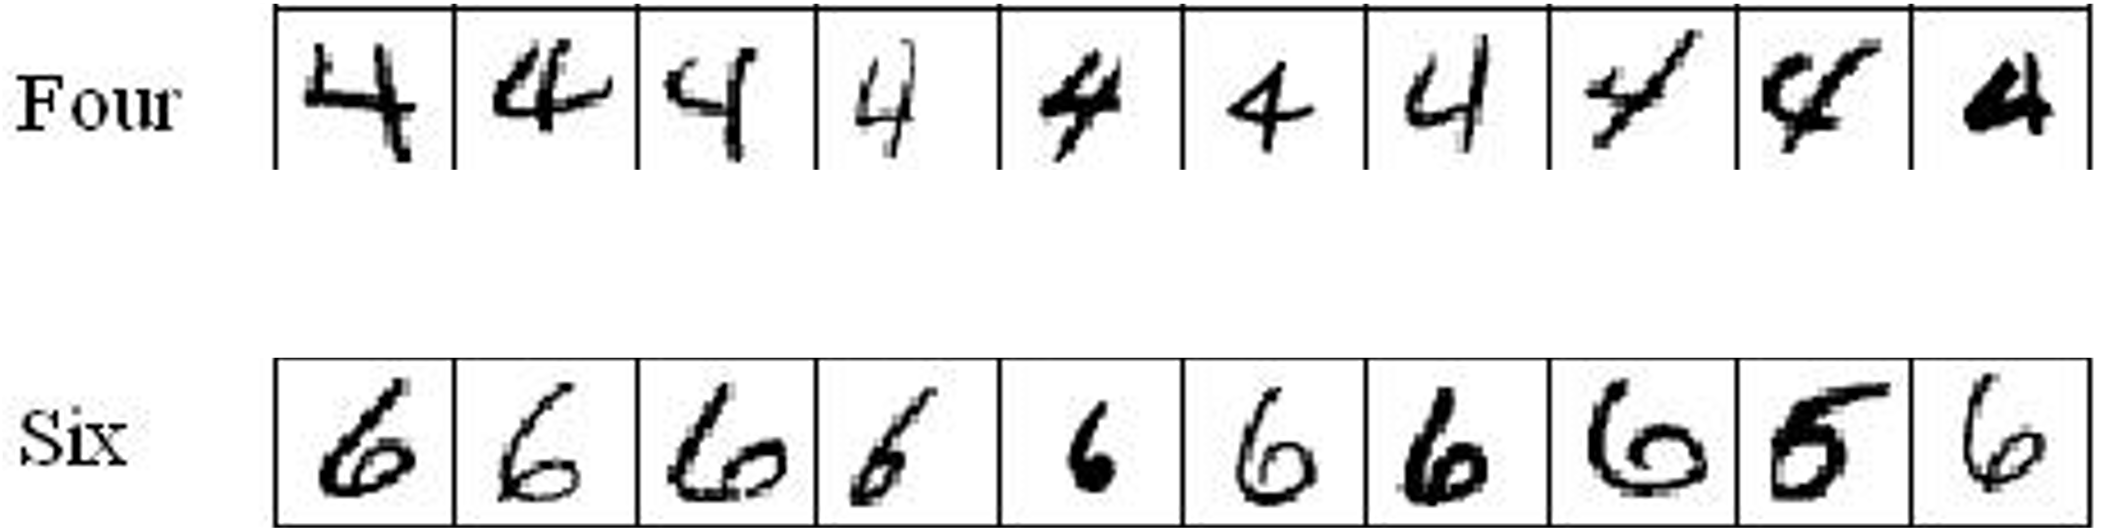
\includegraphics[width=0.60\textwidth]{Topic06fig04.png}
    \caption{Handwritten digits with significant intra-class and inter-class variation.}
  \end{figure}
\end{frame}

\begin{frame}{Higher-Dimensional Linear Separability}
  \justifying
  \begin{conceptbox}{Core Idea}
    Map input to a transformed feature space:
    \[
      \Phi:\mathbb{R}^D\rightarrow\mathbb{R}^{D_k},\quad D_k>D.
    \]
    Learn a linear separator in transformed space.
  \end{conceptbox}
\end{frame}

\begin{frame}{Polynomial Lift Example}
  \justifying
  \[
    \Phi\left(\begin{bmatrix}x_1\\x_2\end{bmatrix}\right)
    =
    \begin{bmatrix}
      x_1^2\\
      \sqrt{2}x_1x_2\\
      x_2^2
    \end{bmatrix}.
  \]
  This maps 2D data into 3D where a plane may separate classes.
\end{frame}

\begin{frame}{2D-to-3D Separation Illustration}
  \justifying
  \begin{figure}[ht]
    \centering
    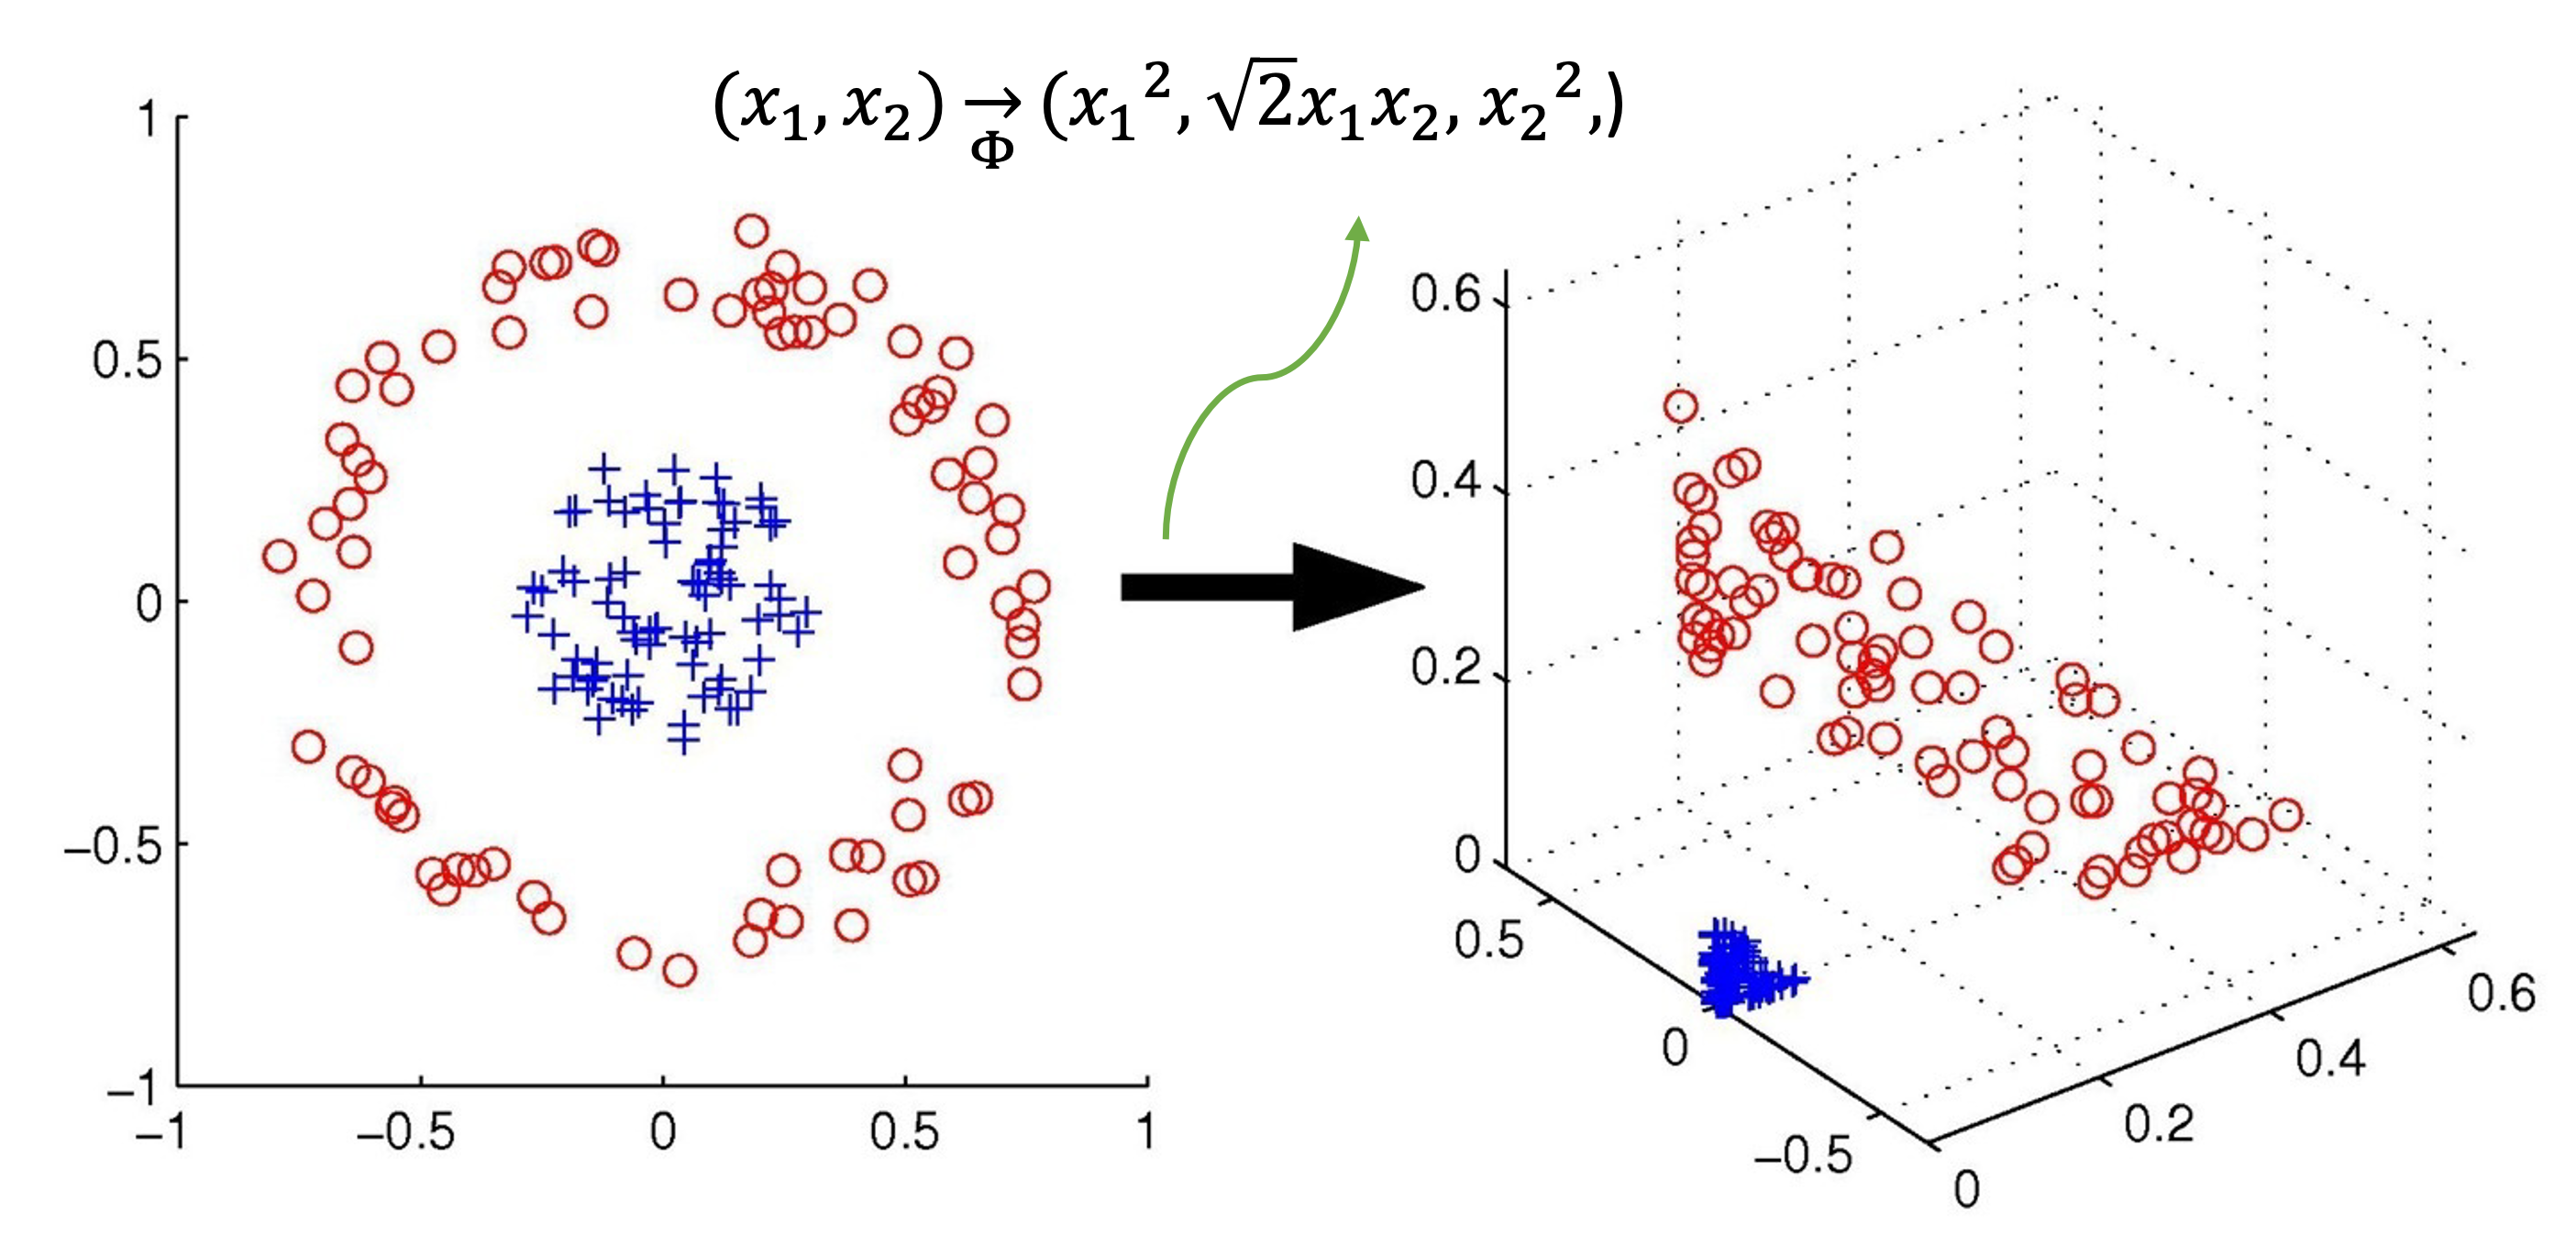
\includegraphics[width=0.62\textwidth]{Topic06fig05.png}
    \caption{Polynomial transformation enabling linear separability in higher dimension.}
  \end{figure}
\end{frame}

\begin{frame}{Linear SVM in Feature Space}
  \justifying
  \[
    u(\Phi(\bm{x})) = \langle\bm{w},\Phi(\bm{x})\rangle.
  \]
  Directly forming $\Phi(\bm{x})$ can be expensive when $D_k$ is large.
\end{frame}

\begin{frame}{Representer Theorem Form}
  \justifying
  \[
    \bm{w} = \sum_{i=1}^N \alpha_i\Phi(\bm{x}_i).
  \]
  Substituting gives
  \[
    u(\bm{x}) = \sum_{i=1}^N \alpha_i\langle\Phi(\bm{x}_i),\Phi(\bm{x})\rangle.
  \]
\end{frame}

\begin{frame}{Kernel Definition}
  \justifying
  \begin{conceptbox}{Kernel Trick}
    \[
      K(\bm{x}_i,\bm{x})=\langle\Phi(\bm{x}_i),\Phi(\bm{x})\rangle.
    \]
    Therefore
    \[
      u(\bm{x})=\sum_{i=1}^N\alpha_i K(\bm{x}_i,\bm{x}).
    \]
  \end{conceptbox}
\end{frame}

\begin{frame}{Norm in Kernel Form}
  \justifying
  \[
    \|\bm{w}\|^2
    =
    \sum_{i=1}^N\sum_{j=1}^N
    \alpha_i\alpha_j K(\bm{x}_i,\bm{x}_j).
  \]
  This avoids explicit high-dimensional coordinates.
\end{frame}

\begin{frame}{Kernel-SVM Objective in $\alpha$}
  \justifying
  \[
    L(\boldsymbol\alpha)
    =
    \frac{1}{2}
    \sum_{i=1}^N\sum_{j=1}^N
    \alpha_i\alpha_jK(\bm{x}_i,\bm{x}_j)
    + C\sum_{j=1}^N h_j.
  \]
\end{frame}

\begin{frame}{Support Vector Sparsity}
  \justifying
  \begin{itemize}
    \item Many $\alpha_i$ become exactly zero after optimization.
    \item Nonzero coefficients correspond to support vectors.
    \item Prediction cost depends on support-vector count.
  \end{itemize}
\end{frame}

\begin{frame}{Single-Item Principle: Why Kernels Work in Practice}
  \justifying
  \begin{itemize}
    \item Kernels decouple representation from explicit coordinates.
    \begin{itemize}
      \item You evaluate similarities, not transformed vectors.
      \item You can model rich nonlinear boundaries with convex training.
      \item Capacity still needs tuning via $C$ and kernel parameters.
    \end{itemize}
  \end{itemize}
\end{frame}

\section{Kernel Functions and Selection}

\begin{frame}{Polynomial Kernel}
  \justifying
  \[
    K(\bm{x},\bm{x}_i)=(\langle\bm{x},\bm{x}_i\rangle+1)^d.
  \]
  \begin{itemize}
    \item Degree $d$ controls boundary flexibility.
    \item Useful when interactions of bounded degree are expected.
  \end{itemize}
\end{frame}

\begin{frame}{Dimension Growth for Polynomial Maps}
  \justifying
  \[
    \dim\bigl(\Phi(\bm{x})\bigr)=\binom{D+d}{d}.
  \]
  \begin{itemize}
    \item Grows combinatorially with $D$ and $d$.
    \item Motivates implicit computation via kernel functions.
  \end{itemize}
\end{frame}

\begin{frame}{RBF Kernel}
  \justifying
  \[
    K(\bm{x},\bm{x}_i)=\exp\bigl(-\gamma\|\bm{x}-\bm{x}_i\|^2\bigr).
  \]
  \begin{itemize}
    \item Produces localized influence around support vectors.
    \item Often strong default for nonlinear tabular tasks.
  \end{itemize}
\end{frame}

\begin{frame}{Interpreting $\gamma$ in RBF}
  \justifying
  \begin{warningbox}{Bandwidth Sensitivity}
    \begin{itemize}
      \item Large $\gamma$: very local decision behavior, overfitting risk.
      \item Small $\gamma$: very smooth boundary, underfitting risk.
    \end{itemize}
  \end{warningbox}
\end{frame}

\begin{frame}{Kernel Selection Workflow}
  \justifying
  \begin{itemize}
    \item Start with linear SVM baseline.
    \item If underfitting, evaluate RBF and polynomial kernels.
    \item Tune $(C,\gamma)$ or $(C,d)$ by cross-validation.
  \end{itemize}
\end{frame}

\begin{frame}{Single-Item Principle: Model Selection Matters}
  \justifying
  \begin{itemize}
    \item Kernel choice should be validated, not assumed.
    \begin{itemize}
      \item Cross-validation balances fit and generalization.
      \item Standardized features stabilize hyperparameter search.
      \item Report both mean and variance across folds.
    \end{itemize}
  \end{itemize}
\end{frame}

\section{SVM Learning and STL-Theoretic View}

\begin{frame}{Why SVM Optimization Is Reliable}
  \justifying
  \begin{itemize}
    \item Linear and kernel SVM objectives are convex.
    \item Convexity supports deterministic global solutions.
    \item Practical solvers use QP/SMO-style methods efficiently.
  \end{itemize}
\end{frame}

\begin{frame}{Training and Testing Risk}
  \justifying
  Define expected testing loss
  \[
    L_{te} = \int l[u(\bm{x}),y] \ dP(\bm{x},y).
  \]
  It is approximated indirectly through training data and complexity control.
\end{frame}

\begin{frame}{VC-Bound Form (Topic Note Expression)}
  \justifying
  \[
    L_{te}
    <
    L_{tr}
    +
    \left[
    \frac{1}{N}
    \left(
      D_{VC}\log\left(\frac{2N}{D_{VC}}+1\right)-\log\left(\frac{\eta}{4}\right)
    \right)
    \right]^{1/2}.
  \]
\end{frame}

\begin{frame}{Interpreting VC-Dimension Impact}
  \justifying
  \begin{itemize}
    \item Higher capacity tends to increase bound looseness.
    \item More samples tighten the confidence term.
    \item Regularization and margin are practical capacity controls.
  \end{itemize}
  \vspace{0.3em}
  \footnotesize
  Source: \href{https://work.caltech.edu/telecourse.html}{Caltech Learning From Data}
\end{frame}

\begin{frame}{Single-Item Principle: Theory-to-Practice Bridge}
  \justifying
  \begin{itemize}
    \item Margin maximization is the operational face of capacity control.
    \begin{itemize}
      \item Geometry explains what model is chosen.
      \item Convex optimization explains why training is stable.
      \item VC-style reasoning explains why the model can generalize.
    \end{itemize}
  \end{itemize}
\end{frame}

\section{Summary}

\begin{frame}{Topic 6 Summary}
  \justifying
  \begin{itemize}
    \item Linear SVMs choose separators by maximizing margin.
    \item Hinge loss and slack variables handle non-separable data.
    \item Kernels make nonlinear SVMs computationally tractable.
    \item Hyperparameters ($C$, $\gamma$, $d$) govern bias-variance balance.
    \item Statistical learning theory motivates margin-based regularization.
  \end{itemize}
\end{frame}

\begin{frame}{What to Practice Next}
  \justifying
  \begin{itemize}
    \item Reproduce linear vs RBF decision boundaries on the same dataset.
    \item Compare support-vector counts across kernels and $C$ values.
    \item Evaluate test performance with repeated cross-validation.
  \end{itemize}
\end{frame}

\end{document}
